%----------------------------------------------------------------------------------------
%    PACKAGES AND THEMES
%----------------------------------------------------------------------------------------

\documentclass[aspectratio=169,xcolor=dvipsnames]{beamer}
\setbeameroption{show notes} %TODO: Thomas a enlever avant la presentation
\usetheme{SimplePlus}

\usepackage{hyperref}
\usepackage{graphicx} % Allows including images
\usepackage{booktabs} % Allows the use of \toprule, \midrule and \bottomrule in tables
\usepackage{array} % Allows >{\centering\arraybackslash} in tabular

%----------------------------------------------------------------------------------------
%    TITLE PAGE
%----------------------------------------------------------------------------------------

\title{Stochastic Optimal Control Matching}
\subtitle{Carles Domingo-Enrich, Jiequn Han, Brandon Amos, Joan Bruna, Ricky T. Q. Chen}

\author{Thomas Mousseau}

% \institute
% {
%     Department of Computer Science and Information Engineering \\
%     National Taiwan University % Your institution for the title page
% }
\date{\today} % Date, can be changed to a custom date

%----------------------------------------------------------------------------------------
%    PRESENTATION SLIDES
%----------------------------------------------------------------------------------------

\begin{document}

\begin{frame}
    % Print the title page as the first slide
    \titlepage
\end{frame}

\begin{frame}{Overview}
    % Throughout your presentation, if you choose to use \section{} and \subsection{} commands, these will automatically be printed on this slide as an overview of your presentation
    \tableofcontents
\end{frame}

%------------------------------------------------
\section{Setup and Preliminaries}

\begin{frame}{Evolution of Generative Models}
    \begin{center}
        \begin{minipage}{0.9\textwidth}
            \vspace{0.3cm}
            
            \small
            \begin{tabular}{@{}l@{\hspace{0.8cm}}p{0.75\textwidth}@{}}
                \textbf{2020} & \textbf{DDPM:} Denoising Diffusion Probabilistic Models interpret generation as reversing a discrete noise-adding process, learning to denoise at each step. They produced high-quality samples but required thousands of slow sampling steps. \\[0.4cm]
                
                \textbf{2021} & \textbf{Score-based Models:} Score-based generative models extended diffusion to continuous-time SDEs, learning the score function ($\nabla_x \log p_t(x)$) to reverse a stochastic diffusion process. This unified diffusion with stochastic control, allowed probability flow ODEs, and sped up sampling. \\[0.4cm]
                
                \textbf{2023} & \textbf{Flow Matching:} Flow matching views generation as learning a deterministic ODE vector field that directly transports a simple distribution (e.g., Gaussian) to data. This removed stochasticity and significantly improved efficiency compared to diffusion/score methods. \\[0.4cm]
            \end{tabular}
            
            \vspace{0.3cm}
        \end{minipage}
    \end{center}
\end{frame}

\begin{frame}{SOC as the Foundation of Generative Models}
    \vspace{-0.3cm}
    \begin{block}{The Core Challenge: Unnormalized Densities}
        Generative models must sample from complex distributions $p_{\text{data}}(x) = \frac{1}{Z} \tilde{p}_{\text{data}}(x)$ where the normalization constant $Z = \int \tilde{p}_{\text{data}}(x) dx$ is intractable to compute. This intractability arises from the curse of dimensionality when integrating over high-dimensional spaces.
    \end{block}

    \vspace{-0.3cm}

    \begin{columns}[t]
        \column{0.48\textwidth}
        \begin{alertblock}{SOC Connection}
            \small
            \textbf{Key Insight:} \\
            Transform tractable distributions (Gaussian) to complex target distributions through \textcolor{blue}{optimal control policies}.
            
            \vspace{0.3cm}
            
            This bridges the gap between:
            \begin{itemize}
                \item Simple sampling (easy)
                \item Complex data distributions (hard)
            \end{itemize}
        \end{alertblock}
        
        \column{0.48\textwidth}
        \begin{block}{Modern Implementations}
            \small
            
            \textbf{Diffusion Models:} \\
            $u_t = -\frac{1}{2}\nabla_x \log p_t(x)$ (denoising)
            
            \vspace{0.2cm}
            \textbf{Score-based Models:} \\
            $u_t = \nabla_x \log p_t(x)$ (score function)
            
            \vspace{0.2cm}
            \textbf{Flow Matching:} \\
            $u_t = \frac{x_1 - x_0}{T-t}$ (deterministic flow)
            
            All learn \textcolor{blue}{optimal control policies} to transport distributions!
        \end{block}
    \end{columns}

    \note{
    \textcolor{blue}{\textbf{Unnormalized Densities:}} The fundamental challenge in generative modeling is sampling from distributions $p(x) = \frac{1}{Z}e^{-E(x)}$ where $Z$ is unknown. SOC provides the mathematical framework to construct sampling procedures. \\
    \vspace{0.1cm}
    \textcolor{orange}{\textbf{Historical Context:}} From Langevin dynamics to modern diffusion models, all major breakthroughs in generative modeling can be understood through the lens of stochastic optimal control theory.
    }
\end{frame}

\begin{frame}{What is a Stochastic Control Problem?}
    
    \begin{block}{Control-Affine Stochastic Differential Equation}
        The general form of a controlled stochastic process:
        \begin{equation}
        dX_t^u = \big(b(X_t^u, t) + \sigma(t)u(X_t^u, t)\big) dt + \sqrt{\lambda}\sigma(t) dB_t
        \end{equation}
    \end{block}

            \vspace{0.3cm}
    
            \textbf{State Process:} $X_t^u \in \mathbb{R}^d$ (system state under control $u$ at time $t$)
            
            \vspace{0.3cm}
            
            \textbf{Drift Term:} $b(X_t^u, t) \in \mathbb{R}^d$ (natural evolution of the system)
            
            \vspace{0.3cm}
            
            \textbf{Control Term:} $\sigma(t)u(X_t^u, t) \in \mathbb{R}^d$ (how control influences the system)
            
            \vspace{0.3cm}
            
            \textbf{Diffusion Coefficient:} $\sigma(t) \in \mathbb{R}^{d \times d}$ (volatility matrix)
            
            \vspace{0.3cm}
            
            \textbf{Noise Process:} $B_t \in \mathbb{R}^d$ (Brownian motion, external randomness)
            
            \vspace{0.3cm}
            
            \textbf{Noise Intensity:} $\lambda > 0$ (controls the strength of stochastic perturbations)

    \note{
    \textcolor{blue}{\textbf{Control-Affine Structure:}} The "control-affine" property means the control $u$ enters linearly (affinely) in the drift term. This is the most general practical form for controlled SDEs, encompassing most applications in finance, robotics, and machine learning. \\    
    \vspace{0.1cm}

   \textcolor{red}{Je dois aussi expliquer l'importance que le steering input ainsi que le noise sont tous les 2 multipliés par sigma(t) ce qui signifie que ...}
    }
\end{frame}

\begin{frame}{The Optimal Control Objective}
    \vspace{-0.3cm}
    
    \begin{block}{Cost Function to Minimize}
        Find the optimal control policy $u^* \in \mathcal{U}$ that minimizes:
        \begin{equation}
        \min_{u \in \mathcal{U}} \mathbb{E}\left[\int_0^T \left(\frac{1}{2}\|u(X_t^u, t)\|^2 + f(X_t^u, t)\right) dt + g(X_T^u)\right]
        \end{equation}
    \end{block}

            \vspace{0.3cm}
    
             \textbf{Control Effort:} $\frac{1}{2}\|u(X_t^u, t)\|^2$ (penalizes large control actions)

            \vspace{0.3cm}

             \textbf{Running Cost:} $f(X_t^u, t)$ (ongoing cost during the process evolution)

            \vspace{0.3cm}

             \textbf{Terminal Cost:} $g(X_T^u)$ (final cost based on end state at time $T$)
            
            \vspace{0.3cm}
            
             \textbf{Control Space:} $\mathcal{U}$ (set of admissible control policies)

    \note{

    }
    
\end{frame}

\begin{frame}{SOC in Practice}

    \vspace{-0.3cm}
    \begin{table}
        \centering
        \small
        \begin{tabular}{>{\centering\arraybackslash}p{0.25\textwidth}|>{\centering\arraybackslash}p{0.22\textwidth}|>{\centering\arraybackslash}p{0.22\textwidth}|>{\centering\arraybackslash}p{0.22\textwidth}}
            \toprule
            \textbf{Aspect} & \textbf{Steering Actuator} & \textbf{Diffusion Models} & \textbf{Flow Models} \\
            \midrule
            \textbf{State $X_t$} & Vehicle position, velocity & Noisy data sample & Clean data sample \\
            \midrule
            \textbf{Control $u_t$} & Steering angle, throttle & Denoising direction & Flow velocity field \\
            \midrule
            \textbf{Dynamics Source} & \textcolor{blue}{Classical physics} (vehicle dynamics) & \textcolor{orange}{Forward noising} process & \textcolor{ForestGreen}{No natural drift} (learnable) \\
            \midrule
            \textbf{Drift $b(X_t,t)$} & Kinematic equations & Predetermined schedule & $b = 0$ (control learns drift) \\
            \midrule
            \textbf{Control Goal} & Reach target safely & Reverse noise process & Transport distributions \\
            \midrule
            \textbf{Noise $\sqrt{\lambda}\sigma dB_t$} & Road disturbances & Brownian motion & Optional stochasticity \\
            \bottomrule
        \end{tabular}
    \end{table}
    
    \vspace{0.3cm}
    
    \begin{alertblock}{Key Insight}
        \textbf{Same mathematical framework, different physics:} SOC unifies vehicle control, generative modeling, and distribution transport under a single theoretical umbrella.
    \end{alertblock}

    \note{
    \textcolor{blue}{\textbf{Steering Actuator:}} The dynamics come from well-established physics - Newton's laws, kinematics, and vehicle dynamics. The control optimizes safety and efficiency. \\
    \vspace{0.1cm}
    \textcolor{orange}{\textbf{Diffusion Models:}} The drift is determined by the forward noising process (e.g., $\beta(t)$), and control learns to reverse this predetermined corruption. \\
    \vspace{0.1cm}
    \textcolor{ForestGreen}{\textbf{Flow Models:}} No natural drift exists - the control $u_t$ directly becomes the drift term, learning the entire velocity field that transports distributions.
    }
\end{frame}

\begin{frame}{Classic Approach to Finding Optimal Control}
    \begin{block}{Optimal Control $u^*$}
        Find the control policy $u^*$ that minimizes the expected cost: $u^* = \arg\min_u J(u)$
    \end{block}
        
    \begin{block}{Hamilton-Jacobi-Bellman (HJB) Equation}
        The classical approach uses the HJB PDE to characterize the value function $V(x,t)$:
        \small
        \begin{equation}
        \frac{\partial V}{\partial t} + \min_u \left[ L(x,u,t) + \frac{\partial V}{\partial x} f(x,u,t) + \frac{1}{2}\text{tr}(\sigma^T \nabla^2 V \sigma) \right] = 0
        \end{equation}
        
        \vspace{0.2cm}
        With boundary condition: $V(x,T) = \Phi(x)$ (terminal cost)
    \end{block}
        
    \begin{alertblock}{The Curse of Dimensionality}
        Classical numerical methods (finite differences, grid-based) become \textcolor{red}{computationally intractable} in high dimensions due to exponential growth in grid size: $\mathcal{O}(N^d)$ where $d$ is dimension.
    \end{alertblock}

    \note{
    \textcolor{blue}{\textbf{HJB Equation:}} The Hamilton-Jacobi-Bellman equation provides the theoretical foundation for solving stochastic optimal control problems by characterizing the value function $V(x,t)$ as the solution to a nonlinear PDE. The optimal control is then $u^*(x,t) = \arg\min_u [\cdots]$ from the HJB equation.
    }
\end{frame}



%TODO: A voir si je veux expliquer ce qu'est une Adjoint Method?!?!??!?!?!?

%TODO: A voir encore si je ne veux pas faire un lien avec RL ou meme directement presente la HJB et demontrer que ls Jacobienne devient difficulement calculate (prix computationnel trop eleve) a plusieurs dimensions
%! For continuous-time problems with low-dimensional state spaces, the standard approach to learn
%! the optimal control is to solve the Hamilton-Jacobi-Bellman (HJB) partial differential equation
%! (PDE) by gridding the space and using classical numerical methods. For high-dimensional problems,
%! a large number of works parameterize the control using a neural network and train it applying a
%! stochastic optimization algorithm on a loss function. These methods are known as Iterative Diffusion
%! Optimization (IDO) techniques [59] (see Subsec. 2.2).

\begin{frame}{Neural PDE Solvers for SOC}
    
    \begin{block}{Core Innovation: Neural ODEs (Chen et al., 2018)}
        \textcolor{blue}{\textbf{Key Insight:}} Replace discrete layers with continuous-time ODEs \\
        $\frac{dh(t)}{dt} = f_\theta(h(t), t)$ where $h(t)$ represents hidden states evolving continuously
    \end{block}

    \vspace{-0.3cm}

    \begin{columns}[t]
        \column{0.48\textwidth}
        \begin{alertblock}{Neural Network Approximation}
            \small
            \textbf{Value Function:}
            \begin{equation}
            V(x,t) \approx V_\theta(x,t)
            \end{equation}
            
            \textbf{Control Policy:}
            \begin{equation}
            u(x,t) \approx u_\phi(x,t)
            \end{equation}
            
            Both parameterized by deep neural networks
        \end{alertblock}
        
        \column{0.48\textwidth}
        \begin{block}{Training Process}
            \small
            \textbf{Physics-Informed Loss:}
            \begin{equation}
            \mathcal{L} = \|HJB_{residual}\|^2 + \|BC_{error}\|^2
            \end{equation}
            
            \textbf{Key Components:}
            \begin{itemize}
                \item \textcolor{blue}{Automatic differentiation} for PDE terms
                \item \textcolor{ForestGreen}{Adjoint method} for gradients
                \item \textcolor{orange}{Stochastic sampling} of $(x,t)$ points
            \end{itemize}
        \end{block}
    \end{columns}
    
    \vspace{0.3cm}
    
    \begin{block}{Advantages Over Classical Methods}
        \begin{itemize}
            \item \textcolor{ForestGreen}{\textbf{High-dimensional scalability:}} No curse of dimensionality
            \item \textcolor{ForestGreen}{\textbf{Mesh-free:}} No spatial discretization required  
            \item \textcolor{orange}{\textbf{Limitation:}} Requires careful tuning and may lack convergence guarantees
        \end{itemize}
    \end{block}

    \note{
    \textcolor{blue}{\textbf{Neural ODEs:}} Chen et al. (2018) showed that residual networks can be interpreted as discretizations of ODEs. This insight led to continuous-depth models and, crucially for our context, neural methods for solving differential equations. \\
    \vspace{0.1cm}
    \textcolor{ForestGreen}{\textbf{Physics-Informed Neural Networks:}} The key is training networks to satisfy the HJB equation through the residual loss, making the physics constraints part of the optimization objective.
    }
\end{frame}

%------------------------------------------------
\section{Stochastic Optimal Control Matching}

\begin{frame}{Reasons behind SOCM (1/2)}
    Many fundamental tasks in machine learning can be naturally cast as stochastic optimal control problems, highlighting the importance of efficient SOC methods.
    
    \vspace{0.4cm}
    
    \begin{block}{Key ML Applications of SOC}
        \begin{itemize}
            \item \textbf{Reward fine-tuning of diffusion and flow models:} Optimizing generation quality using reward signals
            
            \vspace{0.2cm}
            
            \item \textbf{Conditional sampling on diffusion and flow models:} Steering generation towards specific conditions or constraints
            
            \vspace{0.2cm}
            
            \item \textbf{Sampling from unnormalized densities:} Efficiently drawing samples from complex, intractable distributions
            
            \vspace{0.2cm}
            
            \item \textbf{Importance sampling of rare events in SDEs:} Computing probabilities of low-probability but critical events
        \end{itemize}
    \end{block}
    
    \vspace{0.3cm}
    
    \begin{alertblock}{Key Insight}
        The prevalence of SOC formulations in modern ML motivates the need for more efficient and stable solving methods.
    \end{alertblock}
\end{frame}

\begin{frame}{Reasons behind SOCM (2/2)}
    Current SOC methods suffer from optimization challenges that limit their effectiveness.
    
    \vspace{0.3cm}
    
    \begin{columns}[t]
        \column{0.48\textwidth}
        \begin{alertblock}{Current SOC Methods}
            \begin{itemize}
                \item Use \textbf{adjoint methods} (like CNFs)
                \item Yield \textbf{non-convex} function landscapes
                \item Difficult optimization with local minima
                \item Unstable training dynamics
            \end{itemize}
        \end{alertblock}
        
        \column{0.48\textwidth}
        \begin{block}{Diffusion Models Success}
            \begin{itemize}
                \item Use \textbf{least-squares loss}
                \item Create \textbf{convex} functional landscapes
                \item Stable and reliable optimization
                \item Excellent empirical performance
            \end{itemize}
        \end{block}
    \end{columns}
    
    \vspace{0.4cm}
    
    \begin{block}{SOCM's Innovation}
        \textbf{Goal:} Develop least-squares loss formulations for SOC problems, combining the expressiveness of stochastic control with the optimization stability of diffusion models.
    \end{block}
\end{frame}


\begin{frame}{SOCM in Context: Optimization Landscapes}
    \vspace{0.5cm}
    \begin{table}
        \centering
        \begin{tabular}{>{\centering\arraybackslash}p{0.25\textwidth}>{\centering\arraybackslash}p{0.35\textwidth}>{\centering\arraybackslash}p{0.35\textwidth}}
            \toprule
            \textbf{Task} & \textbf{Non-convex} & \textbf{Least Squares} \\
            \midrule
            Generative Modeling & Maximum Likelihood CNFs & Diffusion models and Flow Matching \\
            Stochastic Optimal Control & Adjoint Methods & \textcolor{red}{\textbf{Stochastic Optimal Control Matching}} \\
            \bottomrule
        \end{tabular}
    \end{table}
\end{frame}

\begin{frame}{Introducing Stochastic Optimal Control Matching}
    SOCM offers a more principled, stable, and accurate way to learn generative dynamics by blending stochastic control theory with modern matching-based generative modeling.
    
    \vspace{0.4cm}
    
    \begin{block}{Key Novel Contributions}
        \begin{enumerate}
            \item \textbf{Controlled Stochastic Process:} Views the generation process as a controlled stochastic process bridging a simple distribution to data.
            
            \vspace{0.2cm}
            
            \item \textbf{Least-Squares Matching:} Learning the control via least-squares matching, a stable and convex regression objective.
            
            \vspace{0.2cm}
            
            \item \textbf{Joint Optimization:} Optimizing control and variance-reducing reparameterization matrices simultaneously, for efficient learning.
            
            \vspace{0.2cm}
            
            \item \textbf{Path-wise Reparameterization:} Introducing a path-wise reparameterization trick, boosting gradient estimation quality.
        \end{enumerate}
    \end{block}
\end{frame}


\begin{frame}{The SOCM Framework (1/3)}
    \small
    \begin{block}{SOCM Loss Function}
        The Stochastic Optimal Control Matching objective is defined as:
        \begin{equation}
        \mathcal{L}_{SOCM}(u, M) := \mathbb{E}\left[\frac{1}{T}\int_0^T \|u(X^v_t, t) - w(t, v, X^v, B, M_t)\|^2 dt \times \alpha(v, X^v, B)\right]
        \end{equation}
    \end{block}

    \begin{block}{Where:}
        \begin{itemize}
            \item $X^v$ is the process controlled by $v$: 
            \begin{equation}
            dX^v_t = (b(X^v_t, t) + \sigma(t)v(X^v_t, t)) dt + \sqrt{\lambda}\sigma(t) dB_t \text{, with } X^v_0 \sim p_0
            \end{equation} 
            \item $u(X^v_t, t)$ is the control policy being learned
            \item $w(t, v, X^v, B, M_t)$ is the target matching function
            \item $\alpha(v, X^v, B)$ is a weighting function
        \end{itemize}
    \end{block}
    \note{Ici, je dois presenter en details la matrice Mt, B ainsi que w. De plus, je veux expliquer l'intuition du path-wise reparameterization trick, a novel
            technique to obtain low-variance estimates of the gradient of the conditional expectation of a functional of
            a random process with respect to its initial value}
\end{frame}

\begin{frame}{The SOCM Framework (2/3)}
    \vspace{-0.3cm}
    
    \begin{block}{Reparameterization Function $w(t, v, X^v, B, M_t)$}
        \small
        The \textcolor{blue}{\textbf{target matching function}} computed via path-wise reparameterization:
        \vspace{-0.2cm}
        \begin{equation}
        \begin{aligned}
        w(t, v, X^v, B, M_t) 
        = \sigma(t)^\top \Bigg(
        &- \int_t^T M_t(s) \nabla_x f(X_s^v, s)\, ds 
           \;-\; M_t(T)\nabla g(X_T^v) \\[4pt]
        &+ \int_t^T \big(M_t(s)\nabla_x b(X_s^v, s) - \partial_s M_t(s)\big)(\sigma^{-1}(s))^\top v(X_s^v, s)\, ds \\[4pt]
        &+ \sqrt{\lambda} \int_t^T \big(M_t(s)\nabla_x b(X_s^v, s) - \partial_s M_t(s)\big)(\sigma^{-1}(s))^\top dB_s
        \Bigg)
        \end{aligned}
        \end{equation}
        
        Where $M_t(s)$ is the \textcolor{ForestGreen}{\textbf{reparameterization matrix}} (learned jointly with $u$)
    \end{block}

\end{frame}
    
\begin{frame}{The SOCM Framework (2/3)}
    
    \begin{block}{Importance Weight $\alpha(v, X^v, B)$}
        \small
        The \textcolor{red}{\textbf{importance sampling weight}} for measure correction:
        \vspace{-0.2cm}
        \begin{equation}
        \begin{aligned}
        \alpha(v, X^v, B) = \exp\!\Bigg(
        &- \frac{1}{\lambda}\int_0^T f(X_t^v, t)\, dt
        - \frac{1}{\lambda} g(X_T^v) \\[4pt]
        &- \frac{1}{\sqrt{\lambda}} \int_0^T \langle v(X_t^v, t), dB_t \rangle
        - \frac{1}{2\lambda} \int_0^T \| v(X_t^v, t) \|^2 dt
        \Bigg)
        \end{aligned}
        \end{equation}

        Incorporates \textcolor{orange}{running costs}, \textcolor{orange}{terminal costs}, and \textcolor{orange}{control effort}
    \end{block}

    \note{
    \textcolor{blue}{\textbf{Reparameterization Matrix $M_t$:}} This matrix enables path-wise reparameterization, a technique to reduce variance in gradient estimation by reparameterizing the stochastic process. It's optimized jointly with the control $u$ to minimize the overall SOCM loss. \\
    \vspace{0.1cm}
    \textcolor{red}{\textbf{Importance Weight $\alpha$:}} This exponential weight corrects for the mismatch between the learned control measure and the optimal control measure. However, it can have high variance when costs are large or in high dimensions, which is the main limitation of SOCM.
    }
\end{frame}


\begin{frame}{SOCM Algorithm}
    \begin{figure}
        \centering
        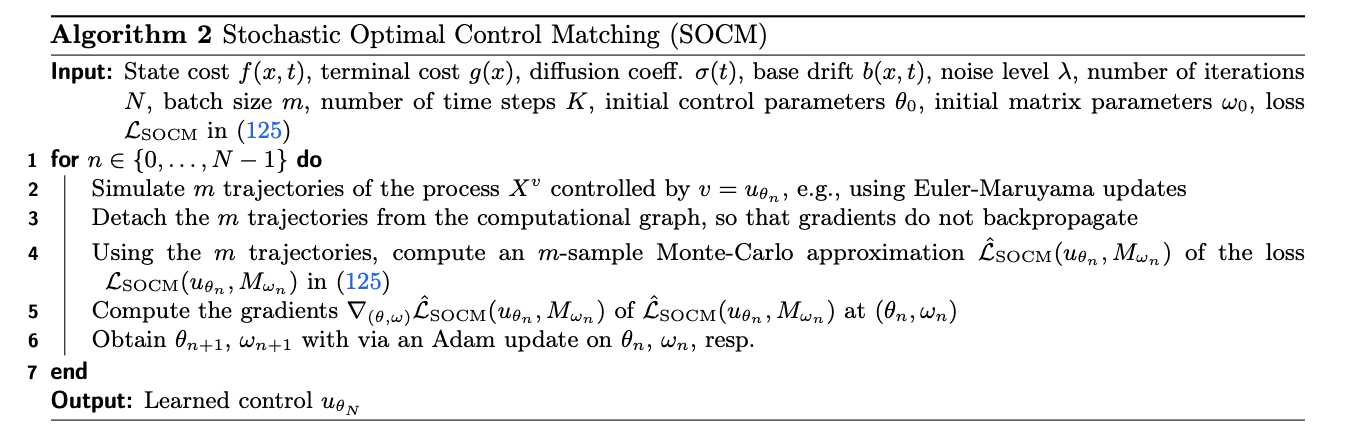
\includegraphics[width=0.95\textwidth]{figures/SOCM_algo.png}
        \caption{Stochastic Optimal Control Matching (SOCM) Algorithm}
    \end{figure}
\end{frame}

%------------------------------------------------

%------------------------------------------------

\section{Experiments and results}
\begin{frame}{Experimental Results (1/2)}
    \begin{figure}
        \centering
        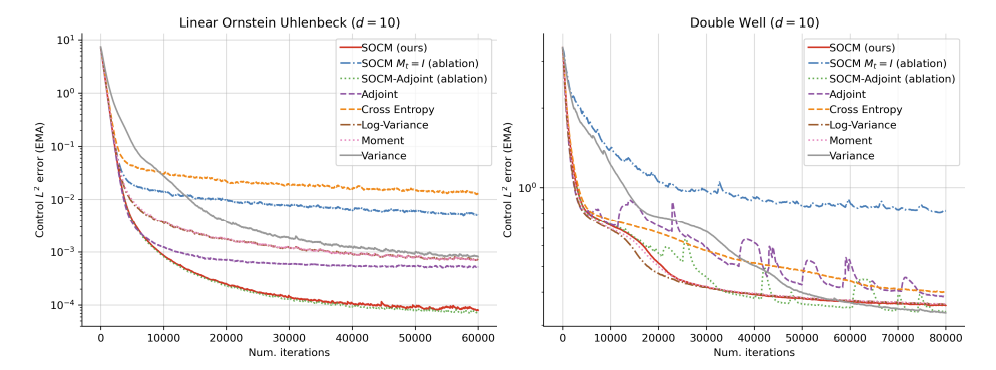
\includegraphics[width=0.95\textwidth]{figures/plots_1.png}
    \end{figure}
\end{frame}

\begin{frame}{Experimental Results (2/2)}
    \begin{figure}
        \centering
        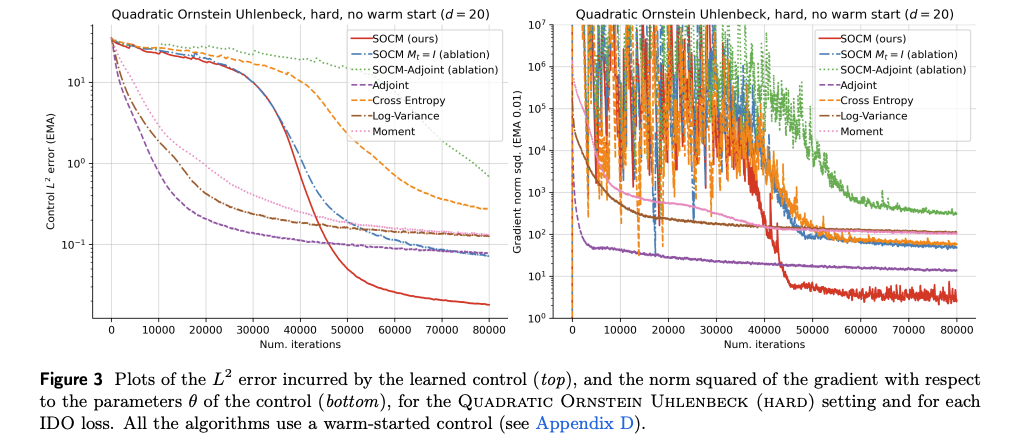
\includegraphics[width=0.95\textwidth]{figures/plots_2.png}
    \end{figure}
    \note{At the end of training, SOCM obtains the lowest L2
        error, improving over all existing methods by a factor of
        around ten. The two SOCM ablations come in second and third by a substantial difference, which underlines
        the importance of the path-wise reparameterization trick.
        \\
        \textcolor{red}{JE DOIS COMPRENDRE CE QUE EST UN ORNSTEIN UHLENBECK PROCESS}
        }
\end{frame}

%------------------------------------------------

%------------------------------------------------
\section{Conclusion}

\begin{frame}{Conclusion}

    \note{The main roadblock when we try to apply SOCM to more challenging problems is that the variance of the
        factor alpha(v, Xv, B) explodes when f and/or g are large, or when the dimension d is high. The control L2 error
        for the SOCM and cross-entropy losses remains high and fluctuates heavily due to the large variance of alpha
        The large variance of alpha is due to the mismatch between the probability measures induced by the learned
        control and the optimal control. Similar problems are encountered in out-of-distribution generalization for
        reinforcement learning, and some approaches may be carried over from that area (Munos et al., 2016).}
\end{frame}

%! so many links to do with RL and Monte Carlo Markov Chains which representent discretized differential equations
%------------------------------------------------

% \begin{frame}{Blocks of Highlighted Text}
%     In this slide, some important text will be \alert{highlighted} because it's important. Please, don't abuse it.

%     \begin{block}{Block}
%         Sample text
%     \end{block}

%     \begin{alertblock}{Alertblock}
%         Sample text in red box
%     \end{alertblock}

%     \begin{examples}
%         Sample text in green box. The title of the block is ``Examples".
%     \end{examples}
% \end{frame}


\begin{frame}{References}
    \footnotesize
    \bibliography{reference.bib}
    \bibliographystyle{apalike}
\end{frame}

%------------------------------------------------

\end{document}